\section{Results}\label{sec:results}
% %**************************************************************
\subsection{Full sequence prediction}\label{subsec:full-sequence-prediction}
The different models we achieved different results, but the most important result is that we settled down an important baseline for the future development of this system.

The encoder-only version of transformer, and feeding the \textit{sequence 3} of Kitti (for more details \S~\ref{sec:kitti}) where the first image is considered as origin, we showed that the model is able to learn a single sequence, in overfitting, and the model fails when trying to overfit a more complex sequence.

The encoder-decoder version we achieved the same results as the previous version, but the model was able to learn the also the \textit{sequence 7} of Kitti, but it fails when we train the model with both \textit{sequence 3} and \textit{sequence 7}.
\begin{figure}[H]
    \centering
    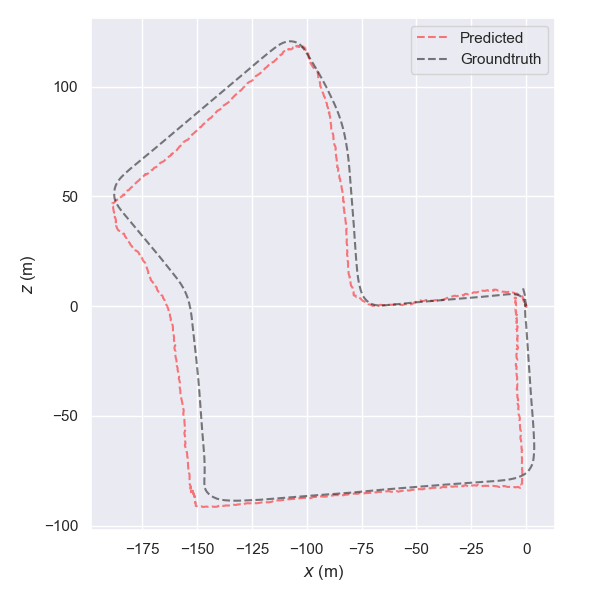
\includegraphics[width=0.5\textwidth]{images/1_4_well_predicted_seq_7}
    \caption{Good prediction sequence 7}\label{fig:well-predicted-seq-7}
\end{figure}

\subsection{Autoregressive models}\label{subsec:autoregressive-model}
We implemented only the encoder-decoder version of the transformer in the autoregressive way, and the results are similar to those of full-sequence predictions.